\documentclass[acmlarge]{acmart}
\usepackage[
    type={CC},           % your choice
    modifier={by-sa},    % your choice
    version={4.0},       % your choice
]{doclicense}            % your choice, see \doclicenseThis below

%\geometry{
%     top=18pt, bottom=14pt, inner=21pt, outer=21pt,
%     paperwidth=5.5in, paperheight=8.5in,
%     }
     
\settopmatter{printacmref=false}
\fancyfoot{}

\makeatletter
\def\@formatdoi#1{}
\def\@permissionCodeOne{miniKanren.org/workshop}
\def\@copyrightpermission{\doclicenseThis} 
\def\@copyrightowner{Copyright held by the author(s).}
\makeatother

\copyrightyear{2019}
\setcopyright{rightsretained}

\acmMonth{8}
\acmArticle{3} % your article number, same as in HotCRP



%% Bibliography style
\bibliographystyle{ACM-Reference-Format}
%% Citation style
%% Note: author/year citations are required for papers published as an
%% issue of PACMPL.
\citestyle{acmauthoryear}   %% For author/year citations


%%%%%%%%%%%%%%%%%%%%%%%%%%%%%%%%%%%%%%%%%%%%%%%%%%%%%%%%%%%%%%%%%%%%%%
%% Note: Authors migrating a paper from PACMPL format to traditional
%% SIGPLAN proceedings format must update the '\documentclass' and
%% topmatter commands above; see 'acmart-sigplanproc-template.tex'.
%%%%%%%%%%%%%%%%%%%%%%%%%%%%%%%%%%%%%%%%%%%%%%%%%%%%%%%%%%%%%%%%%%%%%%


%% Some recommended packages.
\usepackage{booktabs}   %% For formal tables:
                        %% http://ctan.org/pkg/booktabs
\usepackage{subcaption} %% For complex figures with subfigures/subcaptions
                        %% http://ctan.org/pkg/subcaption
\usepackage{multirow}




\usepackage{listings}
\lstdefinelanguage{ocanren}{
keywords={run, conde, fresh, let, in, match, with, when, class, type,
object, method, of, rec, repeat, until, while, not, do, done, as, val, inherit,
new, module, sig, deriving, datatype, struct, if, then, else, open, private, virtual, include, success, failure,
true, false},
sensitive=true,
commentstyle=\small\itshape\ttfamily,
keywordstyle=\textbf,%\ttfamily\underline,
identifierstyle=\ttfamily,
basewidth={0.5em,0.5em},
columns=fixed,
mathescape=true,
fontadjust=true,
literate={fun}{{$\lambda$}}1 {->}{{$\to$}}3 {===}{{$\equiv$}}1 {=/=}{{$\not\equiv$}}1 {|>}{{$\triangleright$}}3 {\\/}{{$\vee$}}2 {/\\}{{$\wedge$}}2 {^}{{$\uparrow$}}1,
morecomment=[s]{(*}{*)}
}

\lstset{
%mathescape=true,
%basicstyle=\small,
%identifierstyle=\ttfamily,
%keywordstyle=\bfseries,
%commentstyle=\scriptsize\rmfamily,
%basewidth={0.5em,0.5em},
%fontadjust=true,
language=ocanren
}

\newcommand{\lstquot}[1]{``\lstinline{#1}''}
\newcommand{\sembr}[1]{\llbracket{#1}\rrbracket}
\newcommand\false{$f\!alse$}
\newcommand\myif{i\!f}


\def\transarrow{\xrightarrow}
\newcommand{\setarrow}[1]{\def\transarrow{#1}}

\def\padding{\phantom{X}}
\newcommand{\setpadding}[1]{\def\padding{#1}}

\def\subarrow{}
\newcommand{\setsubarrow}[1]{\def\subarrow{#1}}

\newcommand{\trule}[2]{\frac{#1}{#2}}
\newcommand{\crule}[3]{\frac{#1}{#2},\;{#3}}
\newcommand{\withenv}[2]{{#1}\vdash{#2}}
\newcommand{\trans}[3]{{#1}\transarrow{\padding{\textstyle #2}\padding}\subarrow{#3}}
\newcommand{\ctrans}[4]{{#1}\transarrow{\padding#2\padding}\subarrow{#3},\;{#4}}
\newcommand{\llang}[1]{\mbox{\lstinline[mathescape]|#1|}}
\newcommand{\pair}[2]{\inbr{{#1}\mid{#2}}}
\newcommand{\inbr}[1]{\left<{#1}\right>}
\newcommand{\highlight}[1]{\color{red}{#1}}
%\newcommand{\ruleno}[1]{\eqno[\scriptsize\textsc{#1}]}
\newcommand{\ruleno}[1]{\mbox{[\textsc{#1}]}}
\newcommand{\rulename}[1]{\textsc{#1}}
\newcommand{\inmath}[1]{\mbox{$#1$}}
\newcommand{\lfp}[1]{fix_{#1}}
\newcommand{\gfp}[1]{Fix_{#1}}
\newcommand{\vsep}{\vspace{-2mm}}
\newcommand{\supp}[1]{\scriptsize{#1}}
\renewcommand{\sembr}[1]{\llbracket{#1}\rrbracket}
\newcommand{\cd}[1]{\texttt{#1}}
\newcommand{\free}[1]{\boxed{#1}}
\newcommand{\binds}{\;\mapsto\;}
\newcommand{\dbi}[1]{\mbox{\bf{#1}}}
\newcommand{\sv}[1]{\mbox{\textbf{#1}}}
\newcommand{\bnd}[2]{{#1}\mkern-9mu\binds\mkern-9mu{#2}}
\newcommand{\meta}[1]{{\mathcal{#1}}}
\newcommand{\dom}[1]{\mathtt{dom}\;{#1}}
%\newcommand{\primi}[2]{\mathbf{#1}\;{#2}}
\renewcommand{\dom}[1]{\mathcal{D}om\,({#1})}
\newcommand{\ran}[1]{\mathcal{VR}an\,({#1})}
\newcommand{\fv}[1]{\mathcal{FV}\,({#1})}
\newcommand{\tr}[1]{\mathcal{T}r_{#1}}
\newcommand{\diseq}{\not\equiv}
\newcommand{\reprfunset}{\mathcal{R}}
\newcommand{\reprfun}{\mathfrak{f}}
\newcommand{\cstore}{\Omega}
\newcommand{\cstoreinit}{\cstore_\epsilon^{init}}
\newcommand{\csadd}[3]{add(#1, #2 \diseq #3)}  %{#1 + [#2 \diseq #3]}
\newcommand{\csupdate}[2]{update(#1, #2)}  %{#1 \cdot #2}
\newcommand{\primi}[1]{\mathbf{#1}}
\newcommand{\sem}[1]{\llbracket #1 \rrbracket}
\newcommand{\ir}{\ensuremath{\mathcal{I\!F}}}

\let\emptyset\varnothing
\let\eps\varepsilon

\sloppy 


\begin{document}

\title[Relational Synthesis of Pattern Matching]{Relational Synthesis of Pattern Matching}    

\titlenote{This work was partially suppored by the grant 18-01-00380 from The Russian Foundation for Basic Research} %% \titlenote is optional;


\author{Dmitry Kosarev}
\email{Dmitrii.Kosarev@pm.me}

\author{Dmitry Boulytchev}
\email{dboulytchev@math.spbu.ru}    

\affiliation{
  \institution{Saint Petersburg State University}
  \country{Russia}                   
}

\affiliation{
  \institution{JetBrains Research}   
  \country{Russia}                   
}


%% Abstract
%% Note: \begin{abstract}...\end{abstract} environment must come
%% before \maketitle command
\begin{abstract}
Effective compilation of pattern matching is important part in a compiler of typed functional language.  We address it via relational synthesis, the algorithm is searching for compiled representation which behaves well on full but finite set of examples and which is minimal. We also describe how to generate full set of examples and our  criteria of minimalism. The approach using relational synthesis seems to be more asily extensible than the default ones.
\end{abstract}


%% 2012 ACM Computing Classification System (CSS) concepts
%% Generate at 'http://dl.acm.org/ccs/ccs.cfm'.
\begin{CCSXML}
<ccs2012>
<concept>
<concept_id>10011007.10011006.10011008.10011009.10011015</concept_id>
<concept_desc>Software and its engineering~Constraint and logic languages</concept_desc>
<concept_significance>500</concept_significance>
</concept>
<concept>
<concept_id>10011007.10011006.10011041.10011047</concept_id>
<concept_desc>Software and its engineering~Source code generation</concept_desc>
<concept_significance>500</concept_significance>
</concept>
</ccs2012>
\end{CCSXML}

\ccsdesc[500]{Software and its engineering~Constraint and logic languages}
\ccsdesc[500]{Software and its engineering~Source code generation(FIXME)}
%% End of generated code


%% Keywords
%% comma separated list
\keywords{relational programming, relational interpreters, search problems}  %% \keywords are mandatory in final camera-ready submission


%% \maketitle
%% Note: \maketitle command must come after title commands, author
%% commands, abstract environment, Computing Classification System
%% environment and commands, and keywords command.
\maketitle

\thispagestyle{empty}

Algebraic data types are essential for typed functional programming and it's difficult to imagine effective compiler without effective compilation of pattern matching. 
There are a few different approaches for compiling pattern mathcing. GHC is using influential paper~\cite{Jones1987}, OCaml is currently based on~\cite{maranget2001} although a work~\cite{maranget2008} can slightly improve effectiveness of generated code. 

Also there are a number of possible extensions of pattern matching itself (guards, non-linear patterns, active patterns) and extensions of possible matchable values (polymorphic variants in OCaml, for example). Although having all these extensions can be helpful for programming in practice, they can complicate compilation schema or make it very difficult to generate effective code. Supporting a large number  of extensions can seriously complicate compiler's implementation too.

We present an approach to pattern matching code generation based on application of relational programming~\cite{TRS,WillThesis} and, in
 particular, relational interpreters~\cite{unified}. We expect that our approach can compile pattern mathcing to competitive code and will be easier to support during adding of new pattern matching extensions.
 
 We use a \emph{relational interpreter} for $\ir$
 
 \[
 eval^o_{\ir}\, (s, p, i)
 \]
 
 Here $s$ and $i$ have the same meaning as in declarative semantics description, $p\in\ir$~--- a syntactic representation of
 a program in $\ir$. The relation $eval^o_{\ir}$ encodes the operational semantics of $\ir$; it holds, if
 evaluating $p$ for $s$ returns $i$. Being relational interpreter, however, $eval^o_{\ir}$ is capable of solving a
 synthesis problem: by a scrutinee $s$ and a number $i$ calculate a program $p$ which makes the relation to hold.
 Within this setting, we can formulate the pattern-matching synthesis problem as follows: \emph{for a given ordered list of patterns $ps$ find a program $p$, such that}
 
 \[
 \forall s\in\mathcal{V},\,\forall i\in\mathbb{N},\,eval^o_{\ir}\, (s, p, i) \wedge\, match (s, ps, i)
 \]
 
 It is rather problematic to directly solve this synthesis problem with existing \textsc{miniKanren} implementations as
 they provide a rather limited support for universal quantification~\cite{eigen,moiseenko}. However, in our concrete
 case there is a simple way to alleviate this problem. Indeed, we may replace universal quantification over $i$ by
 a finite conjunction, as the length of $ps$ is known at the synthesis time. As for the quantification over $s$, for
 any concrete $ps$ we may precompute a \emph{complete set of examples} $\mathcal{E}(ps)\subseteq\mathcal{V}$ with the following
 property:
 
 \[
 \forall i\in\mathbb{N},\,(\forall s\in\mathcal{E}(ps),\,match\, (s, ps, i) \Leftrightarrow \forall s\in\mathcal{V},\,match\, (s, ps, i))
 \]
 
 It easy to see, that for arbitrary $ps$ there exists a finite complete set of examples (indeed, any pattern describes the ``shape''
 of a scrutinee up to some finite depth, beyond which all scrutinees become indistinguishable). Thus, for a given $ps$ we may
 completely eliminate the quantification, reformulating the synthesis problem as
 
 \[
 \bigwedge_{i\in[1\dots|ps|]}\,\bigwedge_{s\in\mathcal{E}(ps)} (eval^o_{\ir}\, (s, p, i) \wedge match\, (s, ps, i))
 \]
 
 We implemented the synthesis framework using \textsc{OCanren}~--- an embedding of \textsc{miniKanren} into \textsc{OCaml}~\cite{ocanren},~---
 and evaluated it on the set of benchmarks, reported in the previous works on \emph{ad-hoc} algorithms for pattern matching
 code generation~\cite{maranget2001,maranget2008}. In comparison with a simplified setting, presented above, our implementation
 deals with a more elaborate pattern matching problem~--- in particular, we support \emph{guard expressions}, name bindings in
 patterns and incorporate a deterministic top-down matching strategy, which is common in functional languages.
 
 Initially, our synthesis did not demonstrate good results. However, we applied the following techniques to improve both the performance
 and the quality of synthesized programs:
 
 \begin{itemize}
 \item we restricted the shape of scrutinees using type information;
 \item we utilized tabling to memoize repeating search steps;
 \item we implemented a pruning technique, which makes the search stop exploring a certain branch if the program, synthesized so far,
   contains too much nesting constructs (this factor can be precomputed by patterns analysis).
 \end{itemize}
 
 With these adjustments, our synthesis framework in a negligible time provides the same results as those reported in the previous works.
 Our future steps include extending the pattern matching language to completely match that of \textsc{OCaml} (for
 now we do not support GADTs), integrate the synthesis into the existing \textsc{OCaml} compiler and evaluate it on a
 set of real-world programs. Another direction is extending the pattern matching language to incorporate features which
 are known to be hard, tedious or error-prone to implement (for example, non-linear patterns).
 
 \begin{comment}
 
 
 Real world modern compilers are obliged to address a few problems which are NP-complete and hence can't have effective
 algorithm to solve them. So, compilers use semi-optimal algorithms to find a decent solution. Optimal algorithms require
 brute force search to get the best solution and  affect compilation speed negatively. In this work we apply relational
 programming -- a convenient DSL for implementing search -- to compilation of pattern matching, one of a kind hard problems for compiler.
 
 The task of compiling pattern matching for typed languages is well presented in literature~\cite{maranget2001,maranget2008}.
 
 
 We test approach on simplified source language $PM$ where scrutinee is a value $\in\mathcal{V}$ of algebraic data type, only wildcards
 and nested constructors are allowed as patterns $\mathcal{P}$ and right hand side of clause is its index. The source language is easy
 extendable by pattern variables and optional pattern guards that test subterms of scrutinee using a function. The semantics of $PM$
 is a function from concrete scrutinee $s$, concrete patterns $pats$ and concrete guards $gs$ to clause indexes, and is denoted
 as $\sem{s,pats,gs}_{PM} = i$.
 
 Compilation scheme translates sentences from $PM$ to $\ir$ language which has constructions for clause indexes and conditions which
 test matchable values for specific constructor. Matchable values can be either a scrutinee, or a projection of matchable value that
 returns one of its field indexed by natural numbers. $\ir$ language is easy extendable by tests for fixed number of pattern guards.
 The semantics is straightforward and is denoted by $\sem{\cdot}_{\ir}$.
 
 We deal with a task of compiling pattern matching as it is a synthesis problem. The goal of algorithm is to synthesize $ideal_\ir$
 for concrete patterns $pats$ and guards that, firstly, will behave the same as original pattern matching for any possible
 scrutinee $s$. Secondly, we want shortest solution because short code usually runs faster. Relational programming~\cite{OCanren}
 will help with that because it has a tendency to generate short answers earlier, although this tendency is not strict.
 
 $$
 \forall s:\; \sem{s; ideal_\ir}_\ir = \sem{s;pats}_{PM}
 $$
 
 To eliminate universal quantifier we use the following observation: for \emph{finite} amount of patterns of \emph{finite} height
 we can generate \emph{finite} amount of examples to test pattern matching semantics. In examples, very deep subterms can have
 any value because they will not be tested during pattern matching. We can reformulate synthesis problem as follows:
 
 $$
 \mid  Examples\mid < \infty\quad \land\quad \left(\forall e \; (e\in Examples)\quad\land \quad\left( \sem{e; ideal_\ir}_\ir = \sem{e;pats}_{PM}\right)\right)
 $$
 
 For plain ADT the approach will generate required examples in finite time, but for GADTs it can diverge because inhabitancy problem
 is semi-decidable~\cite{garrigue2017gadts}(chapter 5). Inhabitants generation as well as synthesis algorithm is
 implemented\footnote{\url{https://github.com/Kakadu/pat-match/}} using relational programming.
 
 Presented approach is good as general description of an idea but require a few tweaks to start working, for example, on presented
 sample~\ref{fig:example1} . Firstly, synthesis procedure in a way as it is described doesn't take types into account, so it is
 useful to give hints about which parts of scrutinee should be checked for which constructors. Second observation says that we
 run $\sem{\cdot}_\ir$ in concrete direction, so it is possible to check periodically count of \texttt{IfTag} constructors in
 result value and prune branches where it becomes too big. Thirdly, synthesis query generates a lot of similar queries, and
 we use tabling to speedup search. All three observations are important, removing one of them leads to visible performance degradation.
 
 The optimal (two \texttt{IfTag}'s) and the semi-optimal solution (three \texttt{IfTag}'s) for~\ref{fig:example1} are described
 in~\cite{maranget2008}. Current implementation generates semi-optimal solution as 28th answer. Before that it generates optimal
 solution (and it's equivalents) three times, other 24 answers are longer and less useful. All tasks (example generation, synthesis
 and printing answers) take 3 seconds, which is unfortunate.
 
 Shortly, we present following contributions
 \begin{itemize}
 \item Code synthesis for pattern matching works after implementing \emph{three optimizations} above.
 \item GADTs, pattern binding and guards works for simple examples, the approach is easy extendable by them.
 \end{itemize}
 
 Future work is
 \begin{itemize}
 \item Discover other optimizations and enable current ones automatically using type information (at the moment we patched synthesis
   algorithm manually for concrete example).
 \item When current implementation tests for \texttt{cons} tag it can't propagate constraint that tag equals to \texttt{nil} to
   the \texttt{else} branch, which partially explains why branch pruning is so useful.
 \item Algorithm for inhabitant generation requires proper formulation and proof.
 \item Apply current synthesis procedure for exhaustiveness checking which will give us \emph{single} procedure for compilation and exhaustiveness checking.
 \item Test the approach on real world problems (embedding to OCaml compiler).
 \end{itemize}
 
 
 \begin{figure}[t]
   \[
   \begin{array}{rcll}
     \mathcal{C} & = & \{ C_1^{k_1}, \dots, C_n^{k_n} \}    &\mbox{(constructors)} \\
     \mathcal{V} & = & \mathcal{C}\,\mathcal{V}^*        &\mbox{(values)}       \\
     \mathcal{P} & = & \_ \mid \mathcal{C}\,\mathcal{P}^*&\mbox{(patterns)}     \\
     \mathcal{M} & = & \bullet \mid \mathcal{M} [\mathbb{N}]&
 
   \end{array}
   \]
 \end{figure}
 
 \begin{figure}
 \centering
 \begin{minipage}{.7\textwidth}
   \centering
 \begin{align*}
 \mathcal{C} =&\; \{ C_1^{k_1}, \dots, C_n^{k_n} \} \\
 \mathcal{V} =&\;  \mathcal{C}\ \mathcal{V}^*\\
 \mathcal{M} =&\;  \mathcal{S} \\
           \mid\; &\; \text{\texttt{Field}}\;  \mathcal{M}\times  \mathbb{N}\\
 \mathcal{P} =&\;  \text{\texttt{Wildcard}} \\
           \mid\; &\; \text{\texttt{Var}}\  Name\\
           \mid\; &\; \text{\texttt{PConstructor}}\  \mathcal{C}\times  \mathcal{P}^*\\
 \ir  =&\; \text{\texttt{Int}}\  \mathbb{N} \\
 %           \mid\; &\;\mathcal{S} \\
            \mid\; &\; \text{\texttt{IfTag}}\; \mathcal{C}\times \mathcal{M}\times \ir\times \ir\\
            \mid\; &\; \text{\texttt{IfGuard}}\ \mathbb{N}\times (Name\times \mathcal{M})^*\times \ir\times \ir\\
 Clause =&\;  \mathcal{P} \times \mathbb{N}? \times \ir
 \end{align*}
   \captionof{figure}{Structure of $PM$ and \ir languages}
 %  \label{fig:test1}
 \end{minipage}%
 \begin{minipage}{.3\textwidth}
   \centering
 \begin{lstlisting}[language=ocaml]
 match s with 
 | ([], _)     -> 1
 | (_, [])     -> 2
 | (_::_,_::_) -> 3
 \end{lstlisting}
   \captionof{figure}{Simple example of pattern matching problem from~\cite{maranget2008}}
 \label{fig:example1}
 \end{minipage}
 \end{figure}
 
 \end{comment}
 

%\section{Searching for Paths in a Graph with a Relational Verifier}
\label{sec:example}

In this section we demonstrate how to solve a concrete problem of searching for paths in a directed graph with a relational verifier. 
A directed graph is a tuple $(N, E, start, end)$, where $N$ is a finite set of \emph{nodes}, $E$ is a finite set of \emph{edges}, functions $start, end : E \rightarrow N$ return a start and an end nodes for a given edge respectively.
A path in a directed graph is a sequence:
\[
\langle n_0, e_0, n_1, e_1, \dots, n_k, e_k, n_{k+1} \rangle
\]

such that 
\[
\forall i \in \{ 0 \dots k \}\; :\; n_i = start\,(e_i) \text{ and } n_{i+1} = end\,(e_i).
\]

The problem of searching for paths in a graph is to find a set $\{ p \mid p \text{ is a path in } g\}$, where $g$ is a graph. 
There~are many concrete algorithms which search for paths in a graph. 
Implementing any of them involves determining in which way to traverse the graph, how to ensure one does not get stuck exploring a cycle in the graph (a cycle is a path in the graph of form $\langle n_0, e_0, \dots, n_k, e_k, n_0 \rangle$), how to ensure one path is not processed multiple times, and so~on. 
A much easier task is to implement a simple verifier, which checks if a sequence is indeed a path in a graph, and generate the path searching routine from it by the relational conversion.

Below is the implementation of the verifier ``\lstinline{isPath}''. 
This function takes as an input a list of nodes ``\lstinline{ns}'' and a graph ``\lstinline{g}''. 
We represent the graph as a list of edges, stipulating there are no parallel edges. 
Each edge $e$ is represented as a pair of nodes $(n, m)$, where $n = start(e)$, $m = end(e)$.
Given $ns = [n_0, \dots, n_{k+1}]$ and a graph $g = [e_0, \dots, e_l]$, the function returns true, if $\exists i_0 \dots i_k \text{ such that } \langle n_0, e_{i_0}, n_1, e_{i_1}, \dots, e_{i_k}, n_{k+1} \rangle$ is a path in $g$.

\begin{lstlisting}[numbers=left,numberstyle=\small,escapeinside={@}{@}]
let rec isPath ns g =
  match ns with
  @\label{lst:isPath_5}@| x$_1$ :: x$_2$ :: xs -> elem (x$_1$, x$_2$) g && isPath (x$_2$ :: xs) g 
  @\label{lst:isPath_4}@| [_]            -> true
\end{lstlisting}

The function ``\lstinline{elem}'' checks if an edge ``\lstinline{e}''  exists in the graph ``\lstinline{g}''. 
We omit the definition of equality check for edges ``\lstinline{eq}'', since it is trivial to implement and is not relevant for the example.

\begin{lstlisting}
let rec elem e g =
  match g with
  | []      -> false
  | x :: xs -> if eq e x then true else elem e xs
\end{lstlisting}

We stipulate that a path must include at least two nodes, since searching for shorter paths is trivial. 
Line~\ref{lst:isPath_5} of the ``\lstinline{isPath}'' definition checks that the first two nodes of the list form an edge of the graph. 
Then it checks that what is left after deleting the first node from the list is still a path in the graph.
Line~\ref{lst:isPath_4} may come off a little counterintuitive, since it states that a path which includes a single arbitrary node is in the input graph.
However we only execute this branch by a recursive call of \lstquot{isPath}, which only happens after we have already ensured with the call to the ``\lstinline{elem}'' function that the said node is in the graph. 

The relational conversion of the verifier function ``\lstinline{isPath}'' generates a relation ``\lstinline{isPath$^o$}'' defined for a path \lstquot{ns}, a graph \lstquot{g} and a boolean value \lstquot{res}, which is true if ``\lstinline{ns}'' is a path in the graph ``\lstinline{g}'' and false otherwise. 
The function ``\lstinline{elem}'' is transformed into a relation ``\lstinline{elem$^o$}'' defined for an edge ``\lstinline{e}'', a graph ``\lstinline{g}'' and a boolean value ``\lstinline{res}'', which is true if ``\lstinline{e}'' is an edge in the graph ``\lstinline{g}'' and false otherwise.
The result of the relational conversion of the functions ``\lstinline{isPath}'' and ``\lstinline{elem}'' is presented below.

\begin{lstlisting}[firstnumber=5, numbers=left,numberstyle=\small,escapeinside={@}{@}]
let rec elem$^o$ e g res = conde [
  (g === nil () /\ res === ^false);
  (fresh (x xs resEq) (
    (g === x % xs) /\ 
    (eq$^o$ e x resEq) /\ 
    (conde [
      (resEq === ^true  /\ res === ^true); 
      (resEq === ^false /\ elem$^o$ e xs res)])))]

let rec isPath$^o$ ns g res = conde [
  (fresh (el) (
    (ns === el % nil ()) /\ 
    (res === ^true));
 @\label{isPatho:fst}@(fresh (x$_1$ x$_2$ xs resElem resIsPath) (
    (ns === x$_1$ % (x$_2$ % xs)) /\ 
    (elem$^o$ (pair x$_1$ x$_2$) g resElem) /\
    (isPath$^o$ (x$_2$ % xs) g resIsPath) /\ 
    (conde [
 @\label{isPatho:die}@     (resElem === ^false /\ res === ^false); 
 @\label{isPatho:lst}@     (resElem === ^true  /\ res === resIsPath)])))]
\end{lstlisting}

Here we use the syntax of \textsc{OCanren}. 
A new relation is defined as a recursive function with the keywords ``\lstinline{let rec}''. 
The body of the relation is a goal created with the following goal constructors. 

\begin{itemize}
    \item Disjunction $g_1 \vee g_2$, where $g_1, g_2$ --- some goals. The two goals are evaluated independently and their results are combined.
    \item Disjunction of goal list \lstinline{conde [$g_1; \ldots; g_n$]}, where $g_1; \ldots; g_n$ --- some goals.
    \item Conjunction $g_1 \wedge g_2$, where $g_1, g_2$ --- some goals. The goal $g_2$ is evaluated only if the evaluation of $g_1$ succeeded; the evaluation of $g_2$ uses the results of $g_1$.
    \item Syntactic unification  $t_1 \equiv t_2$, where $t_1, t_2$ --- some terms. Unification is a basic goal constructor. If $t_1$ and $t_2$ can be unified, the goal is considered successful and failed otherwise. 
    \item Relation call $r^n t_1 \dots t_n$ where $r^n$ is a name of some $n$-ary relation, and $t_i$ are terms. 
    \item To introduce fresh variables into scope, one should use $\textbf{fresh} \; (\overline{x}) \; g$, where $\overline{x}$ is a list of variable names.
\end{itemize}

Besides goal constructors we use some syntactic sugar for values and lists. 
``\lstinline{^}'' is used to transform a value into a logic value. 
The empty list is represented as ``\lstinline{nil ()}'', and to construct a new list from a value ``\lstinline{h}'' and a list ``\lstinline{t}'' we use ``\lstinline{h % t}''.
A tuple of ``\lstinline{x}'' and ``\lstinline{y}'' is created with ``\lstinline{pair x y}''.

Regrettably, this relational interpreter suffers from poor performance. 
Query ``\lstinline{isPath$^o$ q <graph> true}'' for path searching takes more than ten minutes even for graphs of 5 nodes. 
This is somewhat expected, considering that the relational conversion generates a relation which can be used for many different queries, which is excessive when any particular query is in question. 
This is, of course, not a desirable behaviour. Fortunately, further transformation of the relation can improve the performance. 

For example, if we consider a query ``\lstinline{isPath$^o$ q <graph> ^true}'', we can simplify lines~\ref{isPatho:fst} through~\ref{isPatho:lst} of its definition. 
First, we notice that, having ``\lstinline{res}'' be equal to ``\lstinline{^true}'', we can safely remove the disjunct in line~\ref{isPatho:die}, after what the whole ``\lstinline{conde}'' becomes unnecessary and can be removed. 
After moving the unifications for ``\lstinline{resElem}'' and ``\lstinline{resIsPath}'' to the top level, we get the following equivalent definition of the ``\lstinline{isPath$^o$}'' relation. 
Note, that the call to the ``\lstinline{elem$^o$}'' relation is done with the last argument being unified with ``\lstinline{^true}'', so further specialization is still possible. 

\begin{lstlisting}[firstnumber=25, numbers=left,numberstyle=\small,escapeinside={@}{@}]
let rec isPath$^o$ ns g res = conde [
  (fresh (el) (
    (ns === el % nil ()) /\ 
    (res === ^true)));
  (fresh (x$_1$ x$_2$ xs resElem resIsPath) (
    (resElem === ^true) /\
    (resIsPath === ^true) /\
    (ns === x$_1$ % (x$_2$ % xs)) /\ 
    (elem$^o$ (pair x$_1$ x$_2$) g resElem) /\
    (isPath$^o$ (x$_2$ % xs) g resIsPath)))]
\end{lstlisting}

The specialized version of the relation is much more performant than the original one.
Before, searching paths of length 5 took more than 10 minutes while the specialized version finds paths of length 10 in the graph with 100 edges in a few seconds. 

This transformation can be performed automatically with conjunctive partial deduction. 
The result of partially deducing the ``\lstinline{isPath$^o$ q p ^true}'', where ``\lstinline{p}'' and ``\lstinline{q}'' are fresh variables is about 40 lines of code long and it has the same performance as the manually transformed relation. 
We omit the transformed program because of the space concerns, but it can be found in the repository\footnote{https://github.com/Lozov-Petr/miniKanren-2019-Relational-Interpreters-for-Search-Problems}.

%\section{Relational conversion}
\label{sec:conversion}

In this section we describe how the relational conversion in the form of \emph{unnesting}~\cite{lozov:miniKanren} is done. 
Unnesting constructs a relational program by a first-order functional program. 

First, a new variable for every subexpression is introduced with the \lstinline{let}-expression. 
Then, all pattern matching and if-expressions are translated into disjunctions, in which unifications are generated for the patterns.
Free variables are introduced into scope with the \lstinline{fresh}.
Every $n$-ary function becomes $(n+1)$-ary relation with the last argument unified with the result.
As a final step, unifications are reordered with relation calls such that to be computed as early as it is possible.

\begin{figure}[h!]
  \centering
  \begin{subfigure}[t]{0.4\textwidth}
    \centering
\begin{lstlisting}
let rec append a b =
  match a with
  | []      -> b
  | x :: xs -> 
    x :: append xs b
\end{lstlisting}
\caption{}
\label{unnesting_example_a}
  \end{subfigure}
  ~
  \begin{subfigure}[t]{0.4\textwidth}
        \centering
\begin{lstlisting}
let rec append a b =
  match a with 
  | []      -> b
  | x :: xs -> 
    let q = append xs b in
    x :: q
\end{lstlisting}
\vspace{-1\baselineskip}
\caption{}
\label{unnesting_example_b}
  \end{subfigure}
  \vskip2mm
  \begin{subfigure}[t]{0.4\textwidth}
        \centering
\begin{lstlisting}
let rec append$^o$ a b c =
  (a === [] /\ b === c) \/
  (fresh (x xs q) (
     (a === x :: xs) /\
     (append$^o$ xs b q) /\
     (c === x :: q))
\end{lstlisting}
\caption{}
\label{unnesting_example_c}
  \end{subfigure}
  ~
  \begin{subfigure}[t]{0.4\textwidth}
        \centering
\begin{lstlisting}
let rec append$^o$ a b c =
  (a === [] /\ b === c) \/
  (fresh (x xs q) (
     (a === x :: xs) /\
     (c === x :: q) /\
     (append$^o$ xs b q))
\end{lstlisting}
\caption{}
\label{unnesting_example_d}
  \end{subfigure}  
\caption{Example of unnesting}
\label{unnesting_example}
\end{figure}

The example of unnesting is shown in Fig.~\ref{unnesting_example}. 
The input functional program is presented in Fig.~\ref{unnesting_example_a}. 
The result of introducing fresh variables for subexpressions is in Fig.~\ref{unnesting_example_b}.
The relational program before the conjuncts are reordered is shown in Fig.~\ref{unnesting_example_c} and the result of the unnesting is presented in Fig.~\ref{unnesting_example_d}.

Note, that the unnesting has limitations: it does not support higher-order functions and partial application. 
A more general method of translation which does not impose the same limitations was developed~\cite{lozov:conversion}. 
Unfortunately, it uses higher-order relations which are not currently supported in conjunctive partial deduction, so we use unnesting. 

The forward execution of the relation mimics the execution of the function from which it was constructed by relational conversion.
This makes forward execution quite efficient, to the detriment of the execution in the backwards direction. 
The unnesting can be modified to improve the performance of  backward execution. 
Let us consider the conversion of a functional conjunction ``\lstinline{f$_1$ x$_1$ && f$_2$ x$_2$}''.

\begin{lstlisting}
fun res ->
  fresh (p) (
    (f$_1$ x$_1$ p) /\
    (conde [
      (p === ^false /\ res === ^false);
      (p === ^true  /\ f$_2$ x$_2$ res)]))
\end{lstlisting}

Mimicking the function evaluation, the forward execution of this code first computes ``\lstinline{f$_1$ x$_1$}''. 
If it fails, then the result ``\lstinline{res}'' is unified with ``\lstinline{false}'', otherwise the second conjunct ``\lstinline{f$_2$ x$_2$}'' is executed and its result is unified with the result. 
This strategy is not efficient in the backward direction, when we know what ``\lstinline{res}'' is. 
The~following relation is much more performant when executed in the backward direction:

\begin{lstlisting}
fun res ->
    conde [
      (res === ^false /\ f$_1$ x$_1$ ^false);
      (f$_1$ x$_1$ ^true    /\ f$_2$ x$_2$ res)]
\end{lstlisting}

In particular, if ``\lstinline{res === ^true}'', both conversions execute ``\lstinline{f$_2$ x$_2$ res}'', but when the first conversion computes ``\lstinline{f$_1$ x$_1$ p}'' with fresh ``\lstinline{p}'', the second executes ``\lstinline{f$_1$ x$_1$ ^true}''. 
Using the second conversion is enough to significantly increase the performance in the backward direction. 
For example, the path search takes several minutes if the first conversion strategy is used, whereas it finishes in less than a second in the second case. 

Choosing the second conversion strategy comes with a price for the forward execution. 
Instead of executing ``\lstinline{f$_1$ x$_1$ p}'', where ``\lstinline{p}'' is fresh, the second strategy executes both ``\lstinline{f$_1$ x$_1$ ^false}'' and ``\lstinline{f$_1$ x$_1$ ^true}''.
In the worst case scenario, when the execution of ``\lstinline{f$_1$}'' does not depend on the last argument, it doubles the number of executions of ``\lstinline{f$_1$}''.

To sum up, by choosing different strategies of the relational conversion we can achieve significant performance improvement. 
There is no single right way of doing the conversion which improves the performance of the execution in every possible direction. 
Choosing a strategy per each relation and each direction manually is not feasible, but it can be achieved with a fully-automatic program transformation, such as conjunctive partial deduction.

%\section{Conjunctive Partial Deduction}
\label{sec:cpd}
Specialization~\cite{jones1993partial} is a natural way to tackle the problem of redundant computations when a part of the input is known. 
A fully-automatic specialization technique developed in the domain of logic programming is called \emph{partial deduction}~\cite{komorowski1982partial, lloyd1991partial}. 
It is related to the supercompilation of functional languages~\cite{gluck1994partial, turchin1986concept}. 
The particular flavour of the partial deduction we are interested in is called \emph{conjunctive partial deduction}~\cite{de1999conjunctive}.
As opposed to the partial deduction, conjunctive partial deduction handles  conjunctions of atoms, thus being able to perform such optimizations as tupling~\cite{hu1997tupling} and deforestation~\cite{wadler1988deforestation}.
Below we demonstrate by example the features of conjunctive partial deduction.

\emph{Deforestation} is a program transformation which gets rid of intermediate data structures. 
The following example demonstrates deforestation. 
Consider a goal ``\lstinline{append$^o$ xs ys ts /\ append$^o$ ts zs rs}'' (note the shared ``\lstinline{ts}''), where ``\lstinline{append$^o$ x y xy}'' describes concatenation, ``\lstinline{nil ()}'' constructs the empty list, and ``\lstinline{h % t}'' constructs a new list from the value ``\lstinline{h}'' and another list ``\lstinline{t}'' (similarly to ``\lstinline{cons}'' in \textsc{Scheme} and ``\lstinline{::}'' in \textsc{OCaml}).

\begin{lstlisting}[label={cpd:appendo}]
let rec append$^o$ x y xy = conde [
  (x === nil () /\ xy === y);
  (fresh (h t ty) (
     (x  === h % t)  /\  
     (xy === h % ty) /\
     (append$^o$ t y ty)))]
\end{lstlisting}

This goal concatenates three lists: ``\lstinline{xs}'', ``\lstinline{ys}'', ``\lstinline{zs}'', constructing an intermediate list ``\lstinline{ts}''. During the execution of this goal, elements of the list ``\lstinline{xs}'' are examined twice: first when ``\lstinline{ts}'' is constructed, and then when the result ``\lstinline{rs}'' is constructed. What is worse, ``\lstinline{ts}'' is only constructed to be immediately deconstructed. Deforestation gets rid of ``\lstinline{ts}'' in this example.  

A better program would be such that does not construct ``\lstinline{ts}'' at all. 
Such a program be generated from the original definition by conjunctive partial deduction and is shown below: 

\begin{lstlisting}[label={cpd:doubleappendo}]
let rec doubleAppend$^o$ xs ys zs rs = conde [
  (xs === nil () /\ append$^o$ ys zs rs);
  (fresh (h t ts) (
     (xs === h % t)  /\  
     (rs === h % ts) /\
     (doubleAppend$^o$ t ys zs ts)))]
\end{lstlisting}


Conjunctive partial deduction is also capable of \emph{tupling}. 
This transformation makes sure that the same data structure is traversed once even if computing several results. 
The following example demonstrates such a case. 

The goal ``\lstinline{maxLength$^o$ xs m l}'' computes both the maximum value of the list ``\lstinline{xs}'' and its length. 
The elements of the list are Peano numbers with ``\lstinline{zero ()}'' as the zero and ``\lstinline{succ}'' as the successor function.
The third argument ``\lstinline{b}'' of the relation ``\lstinline{le$^o$ x y b}'' is ``\lstinline{^true}'' if ``\lstinline{x}'' is less or equal than ``\lstinline{y}'', and ``\lstinline{^false}'' otherwise. The relation ``\lstinline{gt$^o$ x y b}'' is similar to ``\lstinline{le$^o$ x y b}'', but it checks for ``\lstinline{x}'' to be greater than ``\lstinline{y}''. 

\begin{lstlisting}[label={cpd:maxandlength}]
let maxLength$^o$ xs m l = max$^o$ xs m /\ length$^o$ xs l

let rec length$^o$ xs l = conde [
  (xs === nil () /\ l === zero ());
  (fresh (h t m) (
    xs === h % t /\ l === succ m /\ length$^o$ t m))]

let max$^o$ xs m = max$_1^o$ xs (zero ()) m

let rec max$_1^o$ xs n m = conde [
  (xs === nil () /\ m === n);
  (fresh (h t) (
    (xs === h % t) /\
    (conde [
      (le$^o$ h n ^true /\ max$_1^o$ t n m); 
      (gt$^o$ h n ^true /\ max$_1^o$ t h m)])))]

let rec le$^o$ x y b = conde [
  (x === zero () /\ b === ^true); 
  (fresh (x$_1$) (
    x === succ x$_1$ /\ y === zero () /\ b === ^false)); 
  (fresh (x$_1$ y$_1$) (
    x === succ x$_1$ /\ y === succ y$_1$ /\ le$^o$ x$_1$ y$_1$ b))]

let rec gt$^o$ x y b = conde [
  (x === zero () /\ b === ^false);
  (fresh (x$_1$) (
    x === succ x$_1$ /\ y === zero () /\ b === ^false));
  (fresh (x$_1$ y$_1$) (
    x === succ x$_1$ /\ y === succ y$_1$ /\ gt$^o$ x$_1$ y$_1$ b))]
\end{lstlisting}


Execution of the goal ``\lstinline{maxLength$^o$ xs m l}'' leads to ``\lstinline{xs}'' being traversed twice. 
There is a way to rewrite the program so that ``\lstinline{xs}'' is traversed once, but this requires fusing together the definitions of ``\lstinline{length$^o$}'' and ``\lstinline{max$^o$}'', which either restricts code reuse, or leads to code duplication. 
A better way is to only fuse the definitions when it is needed, and do it automatically by employing tupling. 

The desirable implementation of the ``\lstinline{maxLength$^o$ xs m l}'' relation is the following (the definitions of ``\lstinline{gt$^o$}'' and ``\lstinline{le$^o$}'' are left out for brevity). It can be achieved with conjunctive partial deduction as well: 

\begin{lstlisting}[label={cpd:maxlen}]
let maxLength$^o$ xs m l = maxLength$_1^o$ xs m (zero ()) l

let rec maxLength$_1^o$ xs m n l = conde [
  (xs === nil () /\ m === n /\ l === zero ());
  (fresh (h t l$_1$)
     (xs === h % t) /\
     (l === succ l$_1$) /\
     (conde [
       (le$^o$ h n /\ maxLength$_1^o$ t m n l);
       (gt$^o$ h n /\ maxLength$_1^o$ t m h l)]))]
\end{lstlisting}

\subsection{CPD for Prolog-like languages}

Initially, conjunctive partial deduction was developed for Prolog-like languages.
Conjunctive partial deduction partially evaluates goals, which are conjunctions of atoms, using two levels of control: local and global~\cite{gluck1996controlling}. The global control determines which atoms are to be partially deduced. The local control~--- what the definitions for the atoms selected at the global control shall be.
Both local and global control construct tree structures which represent the input program. 

Local control constructs finite SLD-trees for conjunctions of atoms. 
The construction is guided with an \emph{unfold} operator: it selects a literal from the leaf of the partially constructed SLD-tree and adds its resolvents as children at each step.
Since, in general, SLD-trees are infinite, a decision to stop unfolding should be made at some point. 
There are several techniques for doing this, the most promising of them combine determinacy and either some well-founded or well-quasi order, such as homeomorphic embedding, or other measures. 

Global control determines the set of the conjunctions for which partial SLD-trees are built.
The important goal of the global control is to ensure termination.
The termination is achieved with the \emph{abstraction}.
If there is a goal which is embedded into the current goal, it points to the possibility of nontermination. 
The embedding tells that there is a certain similarity between the two goals, and if a current goal keeps being processed, then their similar subpart will appear again and again, causing nontermination.
Whenever the embedding goals are detected, the current goal is abstracted to remove the common subgoal from consideration. 

When the partial deduction is done, the only thing left is to construct the \emph{residual program}.
The clauses are generated from a partial SLD-tree, one tree per conjunction at the global level. 
A conjunction is uniquely \textit{renamed} to give a name for the predicate being defined. 
All free variables of the root of the tree become arguments of the predicate. 
For each non-failing path in the SLD-tree a clause is generated: a substitution collected along the path is substituted into the head of the clause, and the body is generated from what is in the leaf. 

\subsection{CPD for \textsc{miniKanren}}

In this section we describe how we adapted conjunctive partial deduction for \textsc{miniKanren}. 
We describe the particular unfolding and generalization strategies as well as discuss how the conjunctive partial deduction had to be modified as a response to the differences between \textsc{Prolog} and \textsc{miniKanren}. 

\subsubsection{Local Control}

Goals in \textsc{miniKanren} are different from those in \textsc{Prolog}-like languages: besides conjunction, disjunction and relation calls, there are explicit unification and  introduction of fresh variables. 
We normalize the input goal so that it was a disjunction of conjunctions of relation calls. 
To do so, we first pop all the fresh variables to the top level (``\lstinline{fresh (x) (p (x) /\ fresh (y) (q(x) \/ r(y, x)))}'' becomes ``\lstinline{fresh (x y) (p(x) \/ q(x) /\ r(y, x))}''). 
Then we transform the goal to be a disjuction of conjunctions of relation calls or unifications. 
All unifications in each conjunction are evaluated to some substitution (or the conjunct is discarded, if some unification fails). 
The normalization allows us to only consider conjunctions of relation calls while doing conjunctive partial deduction.

The local control constructs the following tree structure which represents the goal:

\begin{lstlisting}
type local_tree = 
    Fail
  | Success of subst
  | Leaf    of goal list * subst
  | Disj    of local_tree list
  | Conj    of local_tree * goal list
\end{lstlisting}

Leaf nodes can be either ``\lstinline{Fail}'', ``\lstinline{Success}'' or ``\lstinline{Leaf}''. 
The ``\lstinline{Fail}'' node is created whenever the evaluation of the current goal fails. 
When the current goal evaluates to some substitution, we create the ``\lstinline{Success}'' node with this substitution. 
The last leaf node is called ``\lstinline{Leaf}'', it corresponds to some partially evaluated goal. 
This type of node contains a substitution which has been computed up to this point, and a residual goal.
The goal in this type of node is then examined at the global level. 

``\lstinline{Disj}'' node corresponds to a disjunction in a goal: its children are the local control trees constructed for all disjuncts. 
The last type of nodes is a ``\lstinline{Conj}'' node. 
It is a transient node, which keeps track of a conjunction being unfolded. 

In general, unfolding replaces some of the relation calls with their bodies and partially evaluates them.
The particular unfolding strategy we adhere to is the following. 
At each step only one relation call is replaced with its body: the leftmost selectable relation call.
The selectable relation call is the one which does not embed any of its predecessors~--- goals which were unfolded in order to get the current goal. 
Embedding here is the modification of the homeomorphic embedding defined for the conjunctions of goals in conjunctive partial deduction literature~\cite{de1999conjunctive}. 
Since using pure embedding to control unfolding leads to hideously big programs, we also allow only one non-deterministic unfold.

\subsubsection{Global Control}

The conjunctions in the ``\lstinline{Leaf}'' nodes are processed at the global level. 
This step is responsible for the termination of the transformation. 
Generally speaking, the danger for nontermination arises whenever we encounter a subgoal which we have encountered before: processing the same thing will lead to itself over and over again. 
To break the vicious circle, one needs to stop unfolding the encountered subgoal, this is what \emph{abstraction} serves for.

The simplest case here is when we come upon the goal which is equal up to variable renaming to any other goal at the global level. 
When this happens, we stop exploring the goal. 
This is called \emph{variant check} in the literature, and it is done both at the global and the local control levels. 

The more complicated case is when a subpart of the goal repeats. 
This case we test with the modification of the homeomorphic embedding relation (strict homeomorphic embedding), initially developed for conjunctions. 
A conjunction $\overline{A}$ is considered embedded into a conjunction $\overline{B}$ when there is an ordered subconjunction within $\overline{A}$, each conjunct of which is embedded into the corresponding conjunct of $\overline{B}$:
\[
\overline{A} = A_0 \wedge A_1 \wedge \dots \wedge A_n \trianglelefteq B_0 \wedge B_1 \wedge \dots \wedge B_m = \overline{B}, \, \myif \, \exists \{ i_0 \dots i_m \mid \forall j.  i_j < i_{j+1} \}: \forall j \in \{0 \dots m\}. A_{i_j} \trianglelefteq B_j 
\]

A single conjunct is embedded into another ($A_i \trianglelefteq B_j$) when the following relation holds and $A_i$ is \emph{not} a strict instance of the second one $B_j$: 
\[
X \trianglelefteq Y, \text{where } X \text{ and } Y \text{ are variables}
\]
\[
f(x_0, x_1, \dots, x_n) \trianglelefteq f (y_0, y_1, \dots, y_n) \Leftrightarrow \forall i \in \{ 0 \dots n \}. x_i \trianglelefteq y_i
\]
\[
f \trianglelefteq g( y_0, y_1, \dots y_m) \Leftrightarrow \exists i \in \{ 0 \dots m \}. f \trianglelefteq y_i
\]

This check determines two major causes of the growth within the conjunctions. 
The conjunction can grow in some argument of a relation call or the number of conjuncts itself can grow. 
To mitigate the first source of the growth, the bigger conjunction can be replaced with a \emph{most specific generalization} of the two conjunctions.
Otherwise we need to \emph{split} the embedded subconjunction from the rest and start processing them separately. 
This process called \emph{abstraction} removes the subconjunctions which cause potential nontermination, and what is left should indeed be processed further.

\subsubsection{Residualization}

After the transformation is finished, a \emph{residual} program is constructed from the global control tree. 
A relation definition is generated for each conjunction at the global level (this is done with the renaming step of the original conjunctive partial deduction).
First, a unique name is given for each conjunction. 
Then free variables of the conjunction are collected to become the arguments of the relation: the constructors and constants are omitted (for example ``\lstinline{f x (succ y) /\ g (zero ()) z}'' becomes ``\lstinline{fG x y z}''.
The body of the definition is generated from the local control tree which corresponds to the conjunction under consideration.
The body is formed as a disjunction of conjunctions for the non-failure nodes of the local control tree. 
A computed substitution is transformed into a conjunction of unifications.
Suitable definitions are chosen for a goal in a leaf, and the conjunction of their applications is generated. 
As a final step we perform redundant argument filtering as described in~\cite{leuschel1996redundant}, and introduce fresh variables where necessary.

\section{Performance Evaluation}
\label{sec:evaluation}

One of our initial goals was to evaluate, what performance impact would choosing
OCaml as a host language make. In addition we spent some efforts in order to implement \miniKanren in
efficient, tagless manner, and, of course, the outcome of this decision also has to be evaluated. 
Since our library generally follows $\mu$Kanren\footnote{https://github.com/jasonhemann/microKanren}, we've chosen it as a reference implementation.
In addition, we took \texttt{faster-miniKanren}\footnote{https://github.com/webyrd/faster-miniKanren}~--- more elaborated 
implementation with a little different search~--- since it implements disequality constraints. 

For the set of benchmarks we took the following problems:

\begin{itemize}
\item \textbf{expo}~--- exponentation $3^5(=243)$ for integers in binary form is calculated relationally;
\item \textbf{logo}~--- the inverse problem $log_3243(=5)$;
\item \textbf{sorto}~--- sorting a list of Peano numbers (shown as example in Section~\ref{sec:examples});
\item \textbf{quines, twines, trines}~--- self/co-evaluating program construction problems from~\cite{Untagged}.
\end{itemize}

Since the last bundle of benchmarks uses disequality constraints (and, hence, $\mu$Kanren is ruled out) we
split all benchmarks into two sets. 

The evaluation was performed on a desktop computer with Intel Core i7-4790K CPU @ 4.00GHz processor and 32GB of memory.
For OCanren \mbox{\texttt{ocaml-4.04.0+frame_pointer+flambda}} was used, for other implementations~--- Chez~Scheme~9.4.1. 
All benchmarks were run in natively compiled mode ten times, then average user time was taken. The results of evaluation
are shown on figures~\ref{eval:first} and~\ref{eval:second}.

The first conclusion, which is rather easy to derive from the results, is that ``taglessless'' indeed matters. Our initial
implementation did not show essential speedup in comparison with $\mu$Kanren (and was even \emph{slower} on the logarithm 
benchmark). The situation was improved drastically, however, when we switched to a tagless version.

Yet, in comparison with \texttt{faster-miniKanren} our implementation is still lagging behind. We did not discover yet the
reasons, and saved this problem for future research.

\begin{figure}[t]
\centering
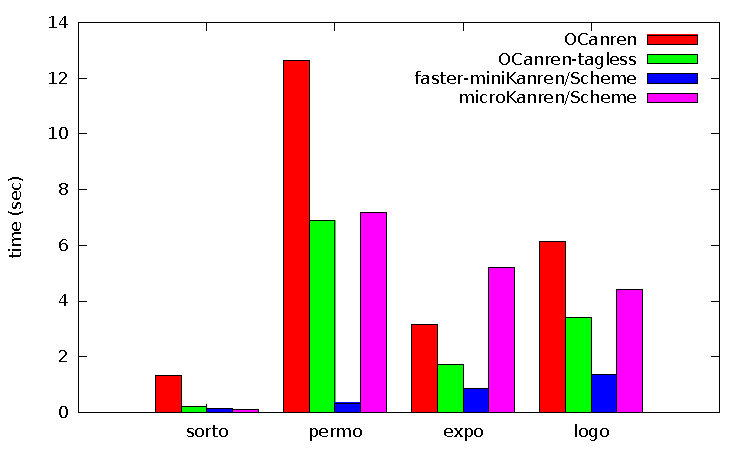
\includegraphics{graph1.pdf}
\caption{The First Set of Benchmarks}
\label{eval:first}
\end{figure}

\begin{figure}[h]
\centering
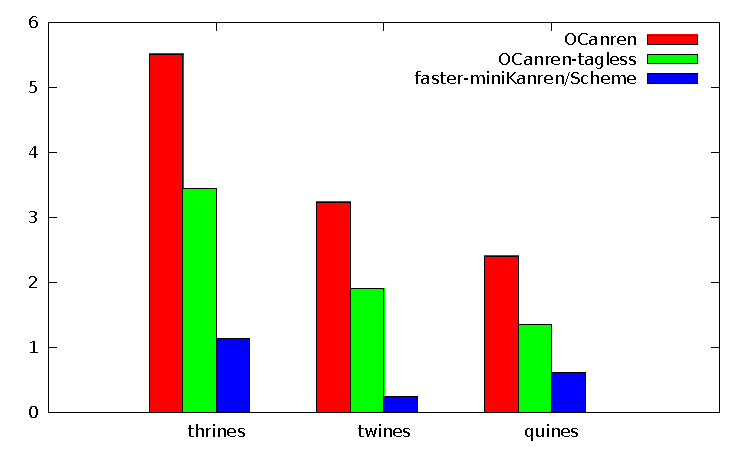
\includegraphics{graph2.pdf}
\caption{The Second Set of Benchmarks}
\label{eval:second}
\end{figure}

\section{Conclusion}

We presented a strongly-typed implementation of \miniKanren for OCaml. Our implementation
passes all tests written for \miniKanren (including those for disequality constraints);
in addition we implemented many interesting relational programs known from
the literature. We claim that our implementation can be used both as a convenient
relational DSL for OCaml and an experimental framework for future research in the area of
relational programming.

%We also want to express our gratitude to William Byrd, who infected us with relational programming,
%and for the extra time he sacrificed as both our tutor and friend.


\begin{comment}
%% Acknowledgments
\begin{acks}                            %% acks environment is optional
                                        %% contents suppressed with 'anonymous'
  %% Commands \grantsponsor{<sponsorID>}{<name>}{<url>} and
  %% \grantnum[<url>]{<sponsorID>}{<number>} should be used to
  %% acknowledge financial support and will be used by metadata
  %% extraction tools.
  This material is based upon work supported by the
  \grantsponsor{GS100000001}{Russian Foundation for Basic Research}{https://www.rfbr.ru/rffi/eng} under Grant
  No.~\grantnum{GS100000001}{18-01-00380} and by the grant from JetBrains Research. 
  %Any opinions, findings, and
  %conclusions or recommendations expressed in this material are those
  %of the author and do not necessarily reflect the views of the
  %National Science Foundation.
\end{acks}
\end{comment}

\bibliography{references}

\end{document}
